\documentclass[a4paper,10pt]{article}
\usepackage[utf8]{inputenc}

\usepackage[english]{babel}
\usepackage[dvinames,table]{xcolor}
\usepackage[compact,small]{titlesec}
\usepackage{booktabs}
\usepackage{multirow}
\usepackage{amsfonts,amsmath,amssymb}
\usepackage{marginnote}
\usepackage[top=1.8cm, bottom=1.8cm, outer=1.8cm, inner=1.8cm, heightrounded, marginparwidth=2.5cm, marginparsep=0.5cm]{geometry}
\usepackage{enumitem}
\setlist{noitemsep,parsep=2pt}
\newcommand{\highlight}[1]{\textcolor{kuleuven}{#1}}
\usepackage{pythonhighlight}
\usepackage{cleveref}
\usepackage{graphicx}
\usepackage{algorithmic}

\newcommand{\nextyear}{\advance\year by 1 \the\year\advance\year by -1}
\newcommand{\thisyear}{\the\year}
\newcommand{\deadlineReport}{January 4, \nextyear{} at 16:00 CET}

\setlength{\parskip}{5pt}
\newcommand{\ReplaceMe}[1]{{\color{blue}#1}}

%opening
\title{JAVA project: Battleship}
\author{Stijn Staring (r0620003)}

\begin{document}
\fontfamily{ppl}
\selectfont{}

\maketitle


\section{The Game}

\subsection{Introduction story}
It is the year 1659 and two rivalling Italian towns are competing for dominance over sea. However, attracted by the wealth of both city states, pirates from the far east have come to raid the prospering towns. In order to repel the attackers the cities have made an agreement to set their difference aside and face the common enemy. The leaders of both cities know however that the whole of Italy is watching them and as soon as the pirates will be defeated, the rivalry will be resumed. In order to gain the most prestige, it is of vital importance to be the clear saviour of Italy and be the one that conflicts the most damage upon the pirates. 

\subsection{Rules}

\paragraph{Setting up the game:}
When the game is started a selection screen will pop up where the players can set their preferences. The rules of the game can again be requested from this frame. During the game the players have to guess where they think the pirate ships are located on a board with a grid layout.Each cell in the grid matches with a certain coordinate defined as $ 5*0 $. Note that the first row and column have the index zero. Under each cell of the grid a part of a pirate boat can be located.\\
The ``\textbf{Choose Ship Placement}'' button allows the players to load a text file that specifies the location of the ships. A template file can be seen in Figure \label{f:template}.If no such file was uploaded, the placement of the ships is automatically done randomly. The first row of the text file should specify the board size by defining respectively the amount of rows and columns of the board. Next, the ships are specified. The order in which this is done is irrelevant, but the ship sizes and names should however comply as shown in Table \ref{t:layoutTextFile}. There should be only four different ships on the board. Also, take into account that the ships can't be separated which means that one direction of a ship has to be chosen and neighbouring cells together form a whole ship. In order to be more robust the system will only take the first two coordinates specified, when the length of the ship is wrong. When other errors occur e.g. the ship has overlap with other ships or lays not in the board, the user will be noted that random placement of the ships will apply.\\

\begin{figure}[h!]
	\begin{center}
		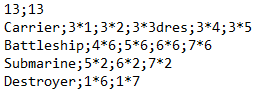
\includegraphics[]{template.PNG}
	\end{center}	
	\caption{An example text file that can be provided to define the ships on the board.}
	\label{f:template}
\end{figure}


\begin{table}[h!]
	\centering
	\begin{tabular}{|p{3cm}|p{2cm}|p{2cm}|}
		\hline
		\textbf{Ship name} & \textbf{Length} & \textbf{Colour}\\ \hline
		Carrier  & $ 5 $ & $ red $\\ \hline
		Battleship  & $ 4 $ & $ green $\\ \hline
		Submarine  & $ 3 $ & $ yellow $\\ \hline
		Destroyer  & $ 2 $ & $ white $\\ \hline
	\end{tabular}
	\caption{Overview of the characteristics of the different ships.}
	\label{t:layoutTextFile}
\end{table}

Next, the ``\textbf{Choose Scoring System}'' button allows the option between an equal score system or an adjusted one. The adjusted score system takes into account that the second player also has information of the move of the first player. Therefore, player one will receive a higher score when a ship is hit. Table \ref{t:scores} gives an overview of the points that can be used. As explained in the Game Play a player receives double points when he hits the last unrevealed cell of the ship.

\begin{table}[h!]
	\centering
	\begin{tabular}{|p{3cm}|p{3cm}|p{3cm}|}
		\hline
		\textbf{Ship name} & \textbf{Standard score} & \textbf{Higher score}\\ \hline
		Carrier  & $ 10 $ & $ 11 $\\ \hline
		Battleship  & $ 15 $ & $ 16 $\\ \hline
		Submarine  & $ 20 $ & $ 21 $\\ \hline
		Destroyer  & $ 25 $ & $ 26 $\\ \hline
	\end{tabular}
	\caption{Overview of the scores that can be used.}
	\label{t:scores}
\end{table}

The spinners that are located on the selection screen can be used to change the dimensions of the board which specifies the amount of cell in the game. The initial value is set to eight and the maximum is thirteen.

\paragraph{Game Play:}\label{s:Gameplay}
When the players start playing the game, a board will appear with grey cells. The players take turn by clicking a grey cell where they think a pirate ship is located. The score and whose turn it is will be indicated at the top of the screen. The players keep clicking the tiles until all four ships have been found whereafter the game automatically ends. When a player hits the last tile of a ship the ship will sink and a double of the points will be received. After a game is finished, the score of the winner will be assessed if it is high enough to be added to the current list of high scores. Only the top five results are being saved. Enjoy! 

\section{Code description}

\subsection{Define classes}
Figure \ref{f:differentClasses} shows the different packages in braun and the classes that they include. Now, a short description is given for each individual class.

\begin{figure}[h!]
	\begin{center}
		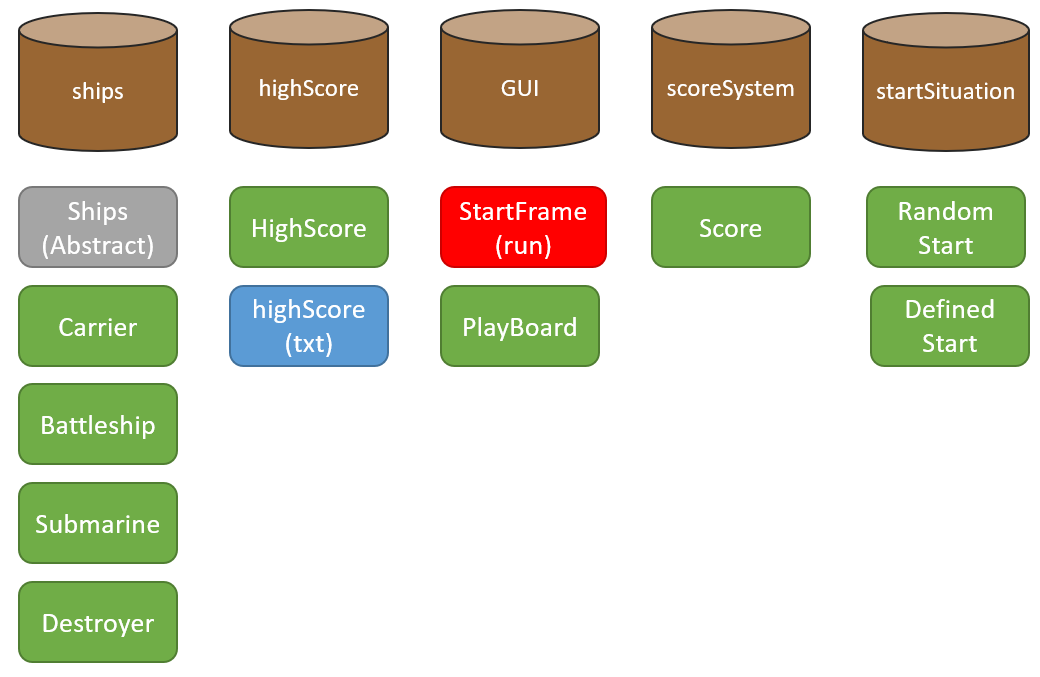
\includegraphics[width=1.0\linewidth]{overviewClasses.PNG}
	\end{center}	
	\caption{An overview of the different packages (Braun), classes (Green), abstract classes (Gray) and text files (Blue).}
	\label{f:differentClasses}
\end{figure}

\newpage

\textbf{Ships}\\
The Ships class is an abstract class that contains the functionality that the specific ships have in common. Functionality that is included is: 
\begin{itemize}
	\item getName 
	\item setStartIndex $ \rightarrow $ coordinate of the first tile on the board
	\item setDirection $ \rightarrow $ direction which the ship is on the board
	\item getLength of the ship $ \rightarrow $ abstract method because the length differs for each ship but already needed in this class
	\item checkShot $ \rightarrow $ is there a ship under the clicked tile or not if so increase the damage
	\item isSunk $ \rightarrow $ is the ship completely damaged
	\item allUsedIndices $ \rightarrow $ get from the start coordinates and direction all the coordinates occupied by the ship
\end{itemize}

\textbf{Carrier/Battleship/Submarine/Destroyer}\\
This class specifies the length of each unique ship and can implements the abstract function getLength.

\textbf{HighScore}\\
At the start of the program the current high scores that were saved in the highScore text file are read in by a buffered reader which provides buffering of data for fast reading. The functionalities that this class overs are:

\begin{itemize}
	\item updateHighScore $ \rightarrow $ this method takes the score of the winner into account and checks if it should be included in the list of high scores
	\item convertToString $ \rightarrow $ converts the ArrayList which stores the high scores to a string format
	\item saveHighScore $ \rightarrow $ when a game is played, the text file on the hard drive is updated
\end{itemize}

\textbf{StartFrame}\\
In the StartFrame class the selection panel is build. This is also the only file that contains a main method.

\textbf{PlayBoard}\\
In the PlayBoard class the play board is build.

\textbf{Score}\\
In this class the scores are given for each hit are assigned. The constructor is overloaded when an adjusted score is used. 
The updateScore method update the score after a player clicked a tile.

\textbf{RandomStart}\\
This class places the ships in a randomly way on the board. Its methods consist out of:

\begin{itemize}
	\item noOverlap
	\item inBoard
	\item generateLegitimatePlace $ \rightarrow $ which produces a set of start coordinates and a direction to define where a ship is placed on the board.
\end{itemize}

\textbf{Define start}\\
Here the user provided text file is read in to define the placement of the ships on the board. It is checked if the user input is feasible. A method defined here is to get the direction of the ship out of two sets of coordinates. 




\subsection{Relations between classes}
\ReplaceMe{Use the words composition and inheritance in your explanation. \\Make a diagram showing the relation between the different classes. Overloading of the constructor is used when defining the different scores used in the game.}
\begin{table}[h!]
	\centering
	
	\begin{tabular}{|p{2cm}|p{1cm}|p{1cm}|p{1cm}|p{1cm}|p{1cm}|p{1cm}|p{1cm}|p{1cm}|p{1cm}|p{1cm}|p{1cm}|}
		\hline
		& \textbf{Sh} & \textbf{Ca}& \textbf{Ba} & \textbf{Su}& \textbf{De} & \textbf{Hi}& \textbf{St} & \textbf{Pl}& \textbf{Sc} & \textbf{Ra}& \textbf{De} \\ \hline
		Ships  &  &  & & & & & & & & & \\ \hline
		Carrier  &  \cellcolor{green!25} &  & & & & & & & & & \\ \hline
		Battleship  &  \cellcolor{green!25} &  & & & & & & & & & \\ \hline
		Submarine  &  \cellcolor{green!25} &  & & & & & & & & & \\ \hline
		Destroyer  &  \cellcolor{green!25} &  & & & & & & & & & \\ \hline
		HighScore  &   &  & & & & & & &\cellcolor{orange!25} & & \\ \hline
		StartFrame  &   &  & & & &\cellcolor{red!25} & & & & & \\ \hline
		PlayBoard  &\cellcolor{red!25}   &  & & & &\cellcolor{red!25} &\cellcolor{orange!25} & & \cellcolor{red!25}& & \\ \hline
		Score  &  \cellcolor{orange!25} &  & & & & & & & & & \\ \hline
		RandomStart  &  \cellcolor{red!25} &  & & & & & & & & & \\ \hline
		DefinedStart  &  \cellcolor{red!25} &  & & & & & & & & & \\ \hline
	\end{tabular}
	\caption{Overview of relations between the different classes. The figure is read from the rows to the columns. extends (Green), composes (Red) or imports (Orange)}
	\label{t:connectionClasses}
\end{table}

\section{Conclusion}
\ReplaceMe{what are the weakenesses of the game.\\ Read the oneNote file to check if anything forgotten.}
















\bibliographystyle{abbrv}
\bibliography{battleshipReferences}

\end{document}